\documentclass[conference]{IEEEtran}
\IEEEoverridecommandlockouts
% The preceding line is only needed to identify funding in the first footnote. If that is unneeded, please comment it out.
\usepackage{cite}
\usepackage{amsmath,amssymb,amsfonts}
\usepackage{algorithmic}
\usepackage{graphicx}
\usepackage{textcomp}
\usepackage{xcolor}
\def\BibTeX{{\rm B\kern-.05em{\sc i\kern-.025em b}\kern-.08em
    T\kern-.1667em\lower.7ex\hbox{E}\kern-.125emX}}
\begin{document}

\title{University of Pretoria \\MIT 805 Group 19\\Group Project Part 1\\
}

\author{\IEEEauthorblockN{Shreya Bharat \\19031786
}
\and
\IEEEauthorblockN{Lerato Mokori\\26834694}
}
}

\maketitle
\section{Introduction}
The TLC Trip Record Dataset contains data collected by the NYC Taxi and Limousine Commission (TLC) on taxi trip records, including information on trip distances, trip fares, and pickup and drop-ff locations. This dataset was chosen to be used for large-scale data processing and analysis, through the use of PySpark. The following report provides a summary of the dataset and its characteristics, the data preparation and preprocessing that was conducted on the dataset, and finally a summary of the exploratory data analysis (EDA) that was conducted on the preprocessed data. 

\section{Dataset provenance and description}
The New York City Taxi TRIP dataset was used for this project. The dataset is provided by the New York City Taxi and Limousine Commission for open access and public use; thus, there are no licensing fees.
Terms of Use: The data may be used for research and educational purposes. There is no warranty provided regarding accuracy or completeness of the data. It is required that users acknowledge the NYC Taxi and Limousine Commission (TLC) as the data source.


\section{Dataset size and characteristics}
Data source: New York City Taxi and Limousine Commission (TLC) Trip Record Data (\usepackage{https://d37ci6vzurychx.cloudfront.net/trip-data})\\

Publication date: Data published monthly by NYC TLC\\

\begin{center}
\begin{tabular}{@{}lll@{}}
\toprule
\textbf{Tier} & \textbf{Actual} \\
\midrule
Raw        & $>$50\,GB documented across four services \\
Working    & 12\,GB downloaded, 139 monthly files \\
Processing & 19\,GB read into Spark after cleaning \\
\bottomrule
\end{tabular}
\end{center}

Format: Apache Parquet, published monthly by NYC TLC.

\section{Data quality and preparation}
The data cleaning was done using Apache Spark to help process the large dataset more efficiently. The monthly files were loaded into Spark Data Frames and standardised to for a consistent schema across the years. Data types were converted to same formats. Duplicate records were removed and observations with missing values on critical fields were excluded. Outlier were removed to avoid working with unrealistic values. Lastly, additional variables were created to support subsequent exploratory analysis. These include trip duration, pickup year, pickup month and pickup day.\\

One of the limitations with using the NYC taxi data is that the data might not be a 100\% accurate as there is no warranty provided regarding accuracy. The dataset only contains New York City and may not be representative of transportation patterns in other regions. The dataset was large, which made it challenging to process and increased processing time. There might be periods affected by temporal disruptions such as COVID19, petrol spikes changing altering client behaviour. Temporal disruptions such as the COVID-19 pandemic could introduce unusual travel behaviour that differs significantly from normal operating conditions. Additionally, correlations observed in the dataset should not be interpreted as causal relationships, as external factors such as weather, economic conditions, tourism activity, and policy changes are not directly captured in the data. It was evident that some important factors that might influence trip patterns were not included in data and therefore not all correlations should be interpreted as cause-and-effect relationships.

\section{Exploratory data analysis of the dataset}
The following section will discuss the exploratory data analysis (EDA) that was conducted on the preprocessed NYC TLC dataset. A total of 139 months of data, spanning 2014-06 to 2025-12, was preprocessed. 95.85\% of the data was retained from the initial working dataset, which initially consisted of 895,333,567 rows of data. The size of the final, preprocessed dataset, is 18.77 GB.\\

Figure \ref{fig1:Average monthly trip volumes} shows the trend in monthly trip volume during the specified time period. The peak number of trips booked in a month was 14,224,018 trips in October 2014, and the lowest recorded month was April of 2020, with a total of 205,234 trips, which is 98.6\% below the recorded peak. The general trend shows a decline in monthly trips, with a step change occurring in 2020. This decline in 2020 can be attributed to the COVID-19 outbreak in the same year, which resulted in many countries imposing travel restrictions and most companies implementing work from home policies. Post COVID-19 saw an initial rise in monthly trips, which eventually stabilised around 4 million trips on average per month. This new average trips per month could also be a reflection of the change in work culture post COVID-19, where many companies adopted remote working as a permanent change to their work policies.\\

Figure \ref{fig2:Average hourly demand} shows the trend in trip volume over a single day, averaged over the entire dataset. For both weekdays and weekends, the percentage of trips taken peaked at 18h00, which is most likely due to work and school commutes. It can be noted that while both graphs peak at the same time, the two curves follow different patterns, with the demand for taxis on weekends increasing later in the day compared to weekdays.\\

Figure \ref{fig3:Trip distribution based on average trip distance} shows the demand for yellow taxis based on the average trip distance. In general, the trend is skewed towards shorter haul trips, with the majority of trips falling below a distance of 5 miles, and approximately 74\% of trips falling below 3 miles. This makes sense given New York's comprehensive rail network, which is more likely to be favoured for longer trips than standard taxis. Figure \ref{fig4:Trip distribution per borough} shows the distribution of trips for the top pickup zones, where the Upper East and Midtown make up 15\% of the top pickup zones. When comparing the average percentage of trips per borough, it was found that 90.6\% of trip pickups were in Manhattan, followed by 6.5\% in Queens.\\ 

\section{The 7 V's of big data}
\subsection{Volume}
The working dataset consisted of approximately 858 million rows of data, after preprocessing and data cleaning, linked to 18.77 GB of data in the form of  Parquet files. Spark was therefore used instead of pandas for handling the data.

\subsection{Velocity}
The average number of trips per day was found to be 202,739 trips, which shows the high frequency at which the data is generated and captured. The busiest day was 2024/11/01, where 574,485 trips were recorded, which is 399 trips captured every minute for the day. Even though the dataset used was data that TLC published in monthly batches, the raw data collected by TLC has to be collected and processed at a very high frequency to provide live feedback to the taxis in operation. 

\subsection{Variety}
The TLC Trip Record Data dataset consists of data spanning four different services, each with a different schema.

\subsection{Value}
The data collected provides significant business value. Data is collected on the revenue generated per trip, which provides business insight into how the four different services are performing and where there may be areas that can be improved to increase the revenue generated. The EDA showed that the revenue per trip generated varied widely, with the highest revenue per vehicle per hour being \$88.35/vehicle-hour at 05:00, and the worst being \$60.29/vehicle-hour at 15:00.

\subsection{Veracity}
Data veracity refers to the accuracy and reliability of the data generated. The preprocessing steps resulted in 95.85\% of the data being retained after it was cleaned, with 37.1 million rows of data having been removed from the raw dataset. This included the removal of duplicate records, record with missing values for key parameters, and major outliers.

\subsection{Variability}
One of the biggest sources of variability in the dataset comes from the fluctuations in data generated between peak hours and downtimes, which results in stark differences in trip fare costs, trip distances, and the speed of trips.

\subsection{Visualisation}
Live dashboards can be used to track peak hours of activity and identify bottlenecks that need to be remedied to improve trip productivity. Spatial mapping in the form of heatmaps can also be used to highlight high-activity boroughs, and the times at which the activity peaks, which could assist with managing where the different services are deployed. 

\section{Potential business/societal value and insights}
Data on the trip fares per hour can be used to improve the pricing model, where trip fares can be predicted by looking at the historical taxi demand per hour, the current fleet availability, and the routes that are most active. This could aid in reducing the gap in revenue generated per trip between the peak and off-peak hours.

\section{GitHub Repository}
The project setup and code can be found in the following GitHub repo: \usepackage{https://github.com/ShreyaB143/MIT805-GroupProject}

\newpage
\clearpage 
\onecolumn 

\section{Appendix} 
\counterwithin{figure}{section} 
\renewcommand{\thefigure}{\Alph{section}.\arabic{figure}} 

\begin{figure}[htbp]
    \centering
    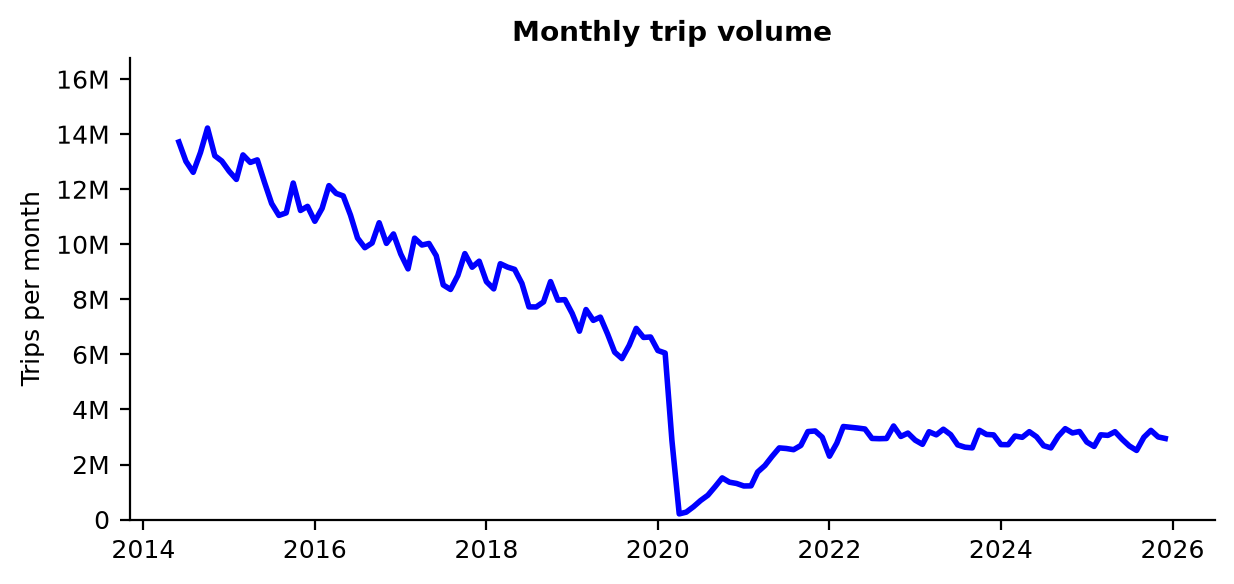
\includegraphics[width=0.8\textwidth]{fig1_monthly_volume.png}
    \caption{Average monthly trip volumes.}
    \label{fig1:Average monthly trip volumes}
\end{figure}

\begin{figure}[htbp]
    \centering
    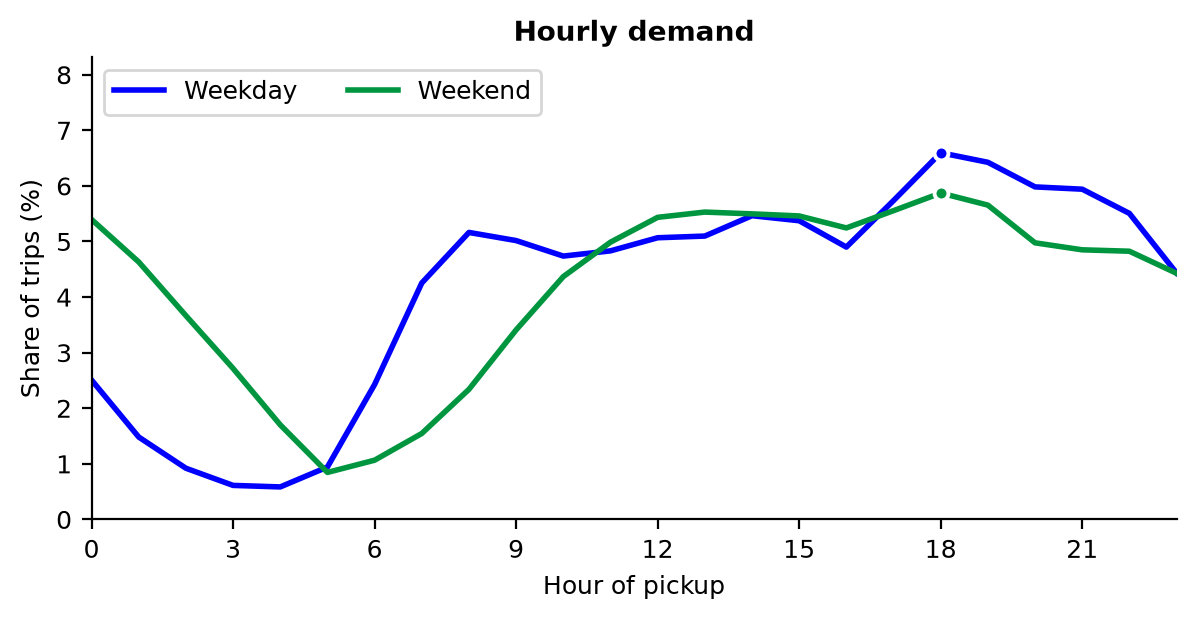
\includegraphics[width=0.8\textwidth]{fig2_hourly_demand.png}
    \caption{Average hourly demand.}
    \label{fig2:Average hourly demand}
\end{figure}

\begin{figure}[htbp]
    \centering
    
\includegraphics[width=0.8\textwidth]{fig3_distance_distribution.png}
    \caption{Trip distribution based on average trip distance.}
    \label{fig3:Trip distribution based on average trip distance}
\end{figure}

\begin{figure}[htbp]
    \centering
    
\includegraphics[width=0.8\textwidth]{fig4_top_zones.png}
    \caption{Trip distribution per borough.}
    \label{fig4:Trip distribution per borough}
\end{figure}


\end{document}
